Este manual tiene como objetivo proporcionarte una guía detallada sobre cómo utilizar todas las características y funcionalidades de nuestro sitio web en dispositivos móviles.

\subsubsection{Requisitos del Sistema}
Antes de comenzar, asegúrate de que tu dispositivo cumple con los siguientes requisitos:

\begin{itemize}
	\item Navegador web móvil actualizado (recomendamos Google Chrome o Mozilla Firefox).
	\item Conexión a Internet estable.
	\item Resolución de pantalla mínima de 375x667 píxeles.
\end{itemize}

\subsubsection{Acceso a la Página Web}
Para acceder a nuestra página web desde tu dispositivo móvil, sigue estos pasos:

\begin{enumerate}
	\item Abre tu navegador web.
	\item En la barra de direcciones, ingresa la URL de nuestro sitio web: www.astour.online.
	\item Presiona Enter.
\end{enumerate}

\subsubsection{Funcionalidades Principales}
A continuación, describiremos las funcionalidades principales de nuestra página web en su versión móvil:

\subsubsection{Inicio de Sesión}
Antes de iniciar sesión deberás solicitar tus credenciales de acceso al administrador del sistema.
Con las credenciales de acceso, sigue estos pasos para iniciar sesión:

\begin{enumerate}
	\item Toca el ícono de menú en la parte superior izquierda de la página de inicio y selecciona la opción “Cuenta” .
	      \begin{figure}[H]
		      \centering
		      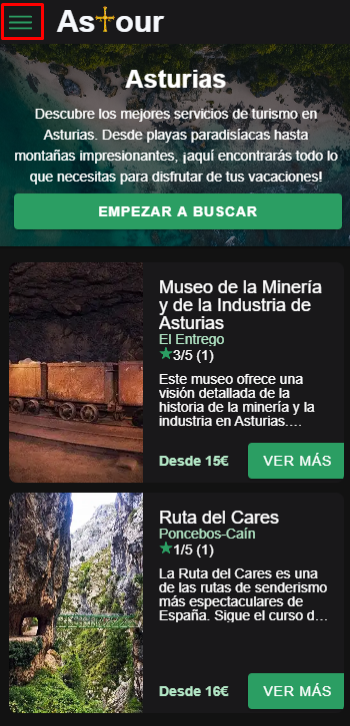
\includegraphics[width=0.3\textwidth]{7-Construccion/Manuales/mobile/menu marcado.png}
		      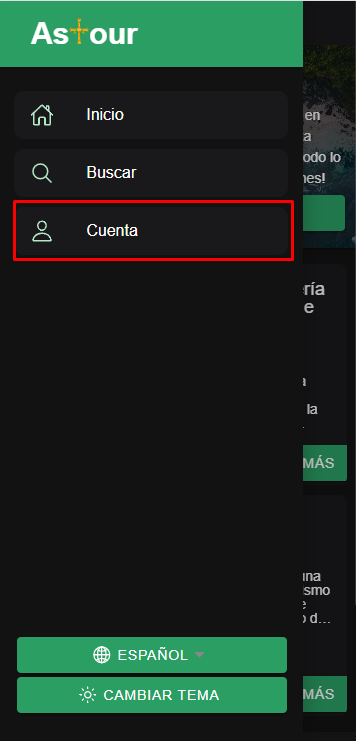
\includegraphics[width=0.3\textwidth]{7-Construccion/Manuales/mobile/cuenta marcado.png}
		      \caption{Inicio de sesión - Despliegue del menú y selección de la opción “Cuenta”.}
	      \end{figure}
	\item Ingresa tu email y contraseña en los campos correspondientes y toca el botón “Iniciar Sesión” para acceder a tu cuenta.
	      \begin{figure}[H]
		      \centering
		      \includegraphics[width=0.3\textwidth]{7-Construccion/Manuales/mobile/iniciar sesión.png}
		      \caption{Inicio de sesión - Selección de la opción “Iniciar Sesión”.}
	      \end{figure}
\end{enumerate}

Al iniciar sesión con éxito, accederás a tu cuenta y podrás comenzar a gestionar tus próximos eventos.

\subsubsection{Exploración de Actividades}
Desde la página de inicio, puedes explorar las actividades pulsando el botón “Empezar a buscar” .
Te llevará a una página donde encontrarás una lista de actividades disponibles, con la opción de filtrar por nombre, por rango de fechas, precio máximo, número de personas, puntuación mínima y idioma.
\begin{figure}[H]
	\centering
	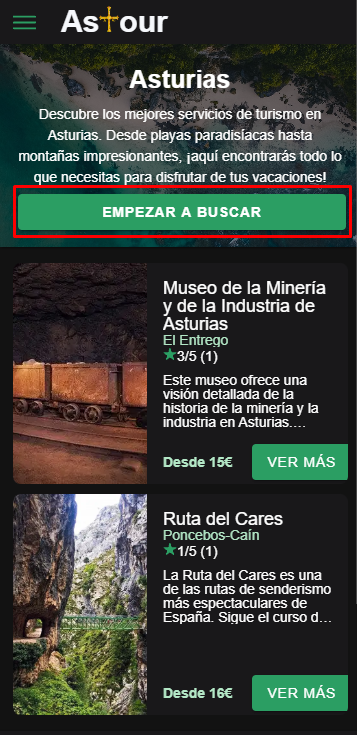
\includegraphics[width=0.3\textwidth]{7-Construccion/Manuales/mobile/empezar a buscar.png}
	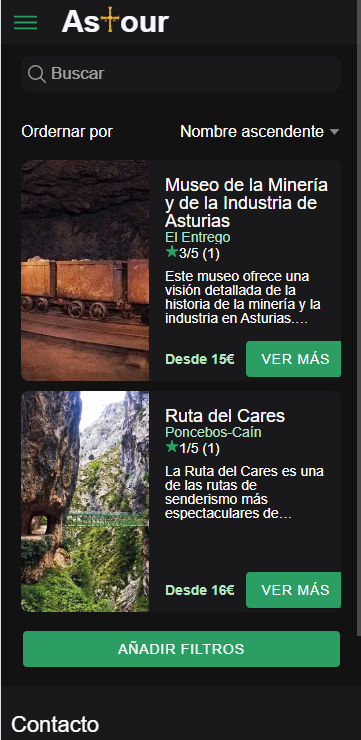
\includegraphics[width=0.3\textwidth]{7-Construccion/Manuales/mobile/lista de actividades.png}
	\caption{Explorar actividades - Redirección a la lista de actividades.}
\end{figure}

Para filtrar por nombre, ingresa el nombre de la actividad en la barra de búsqueda superior.
A los 3 segundos de haber dejado de escribir, se mostrarán las actividades que coincidan con el nombre ingresado.
\begin{figure}[H]
	\centering
	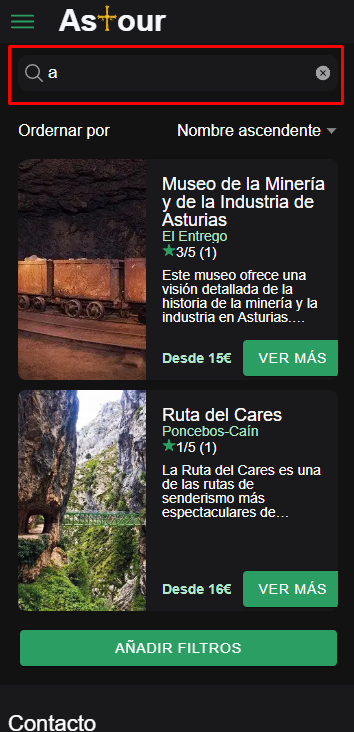
\includegraphics[width=0.3\textwidth]{7-Construccion/Manuales/mobile/busqueda por nombre.png}
	\caption{Explorar actividades - Búsqueda de actividades por nombre.}
\end{figure}

Para filtrar por una características más específicas, toca el botón “Filtros” que se encuentra en la parte superior derecha de la pantalla.
Se abrirá un menú con las opciones de filtrado disponibles.
\begin{figure}[H]
	\centering
	\includegraphics[width=0.3\textwidth]{7-Construccion/Manuales/mobile/añadir filtros.png}
	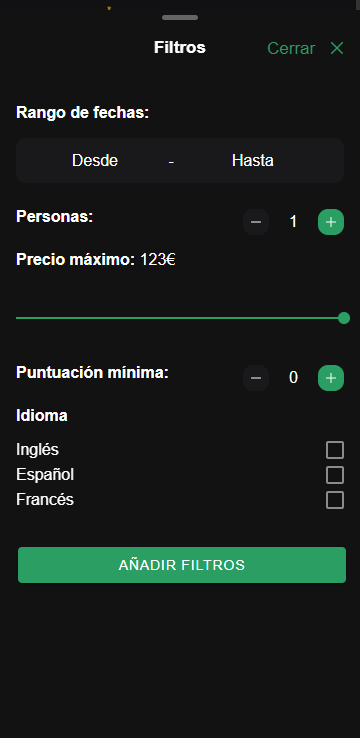
\includegraphics[width=0.3\textwidth]{7-Construccion/Manuales/mobile/menu vacio filtros.png}
	\caption{Explorar actividades - Añadir filtros.}
\end{figure}

Para filtrar por rango de fechas, selecciona las fechas de inicio y fin en los campos correspondientes.
\begin{figure}[H]
	\centering
	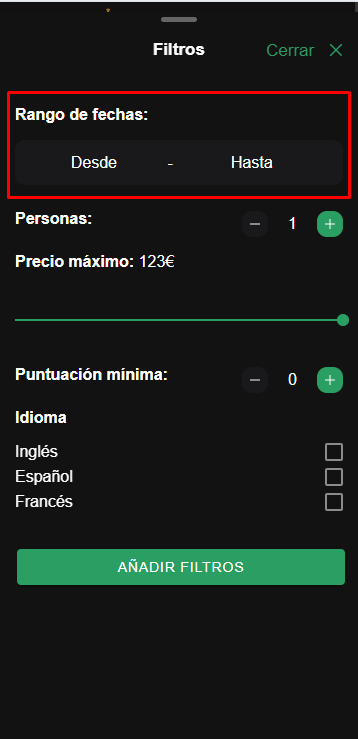
\includegraphics[width=0.3\textwidth]{7-Construccion/Manuales/mobile/filtro fechas.png}
	\caption{Explorar actividades - Filtro de fechas.}
\end{figure}
Para filtrar por precio máximo, ajusta el control deslizante.
\begin{figure}[H]
	\centering
	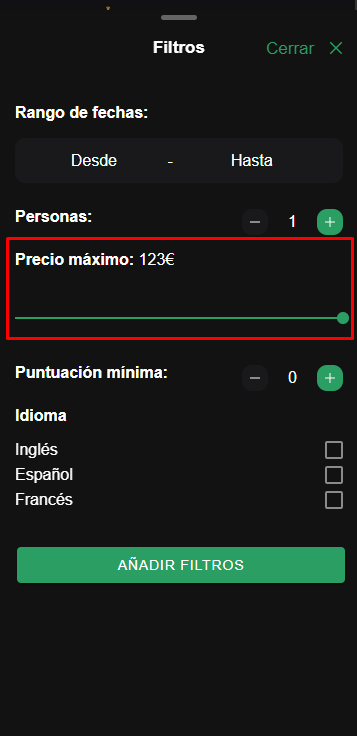
\includegraphics[width=0.3\textwidth]{7-Construccion/Manuales/mobile/filtro precio.png}
	\caption{Explorar actividades - Filtro de precio.}
\end{figure}
Para filtrar por número de personas, utiliza los botones de incremento y decremento.
\begin{figure}[H]
	\centering
	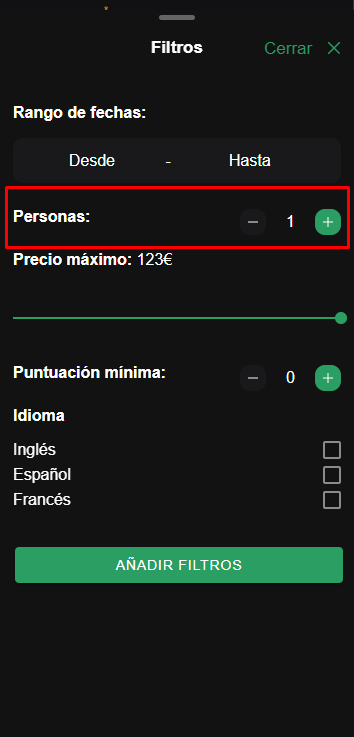
\includegraphics[width=0.3\textwidth]{7-Construccion/Manuales/mobile/filtro personas.png}
	\caption{Explorar actividades - Filtro de personas.}
\end{figure}
Para filtrar por puntuación mínima, utiliza los botones de incremento y decremento.
\begin{figure}[H]
	\centering
	\includegraphics[width=0.3\textwidth]{7-Construccion/Manuales/mobile/filtro puntuación.png}
	\caption{Explorar actividades - Filtro de puntuación.}
\end{figure}
Para filtrar por idioma, selecciona los idiomas deseados tocando las casillas correspondientes.
\begin{figure}[H]
	\centering
	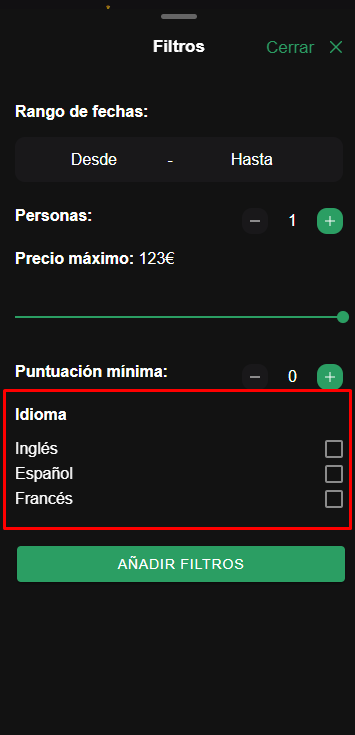
\includegraphics[width=0.3\textwidth]{7-Construccion/Manuales/mobile/filtro idioma.png}
	\caption{Explorar actividades - Filtro de idioma.}
\end{figure}

Para aplicar los filtros específicos, pulsa el botón “Añadir filtros” que se encuentra en la parte inferior de la pantalla.
En el caso que desees modificar los filtros aplicados, vuelve a pulsar el botón “Añadir filtros” después de haber seleccionado los filtros deseados.
\begin{figure}[H]
	\centering
	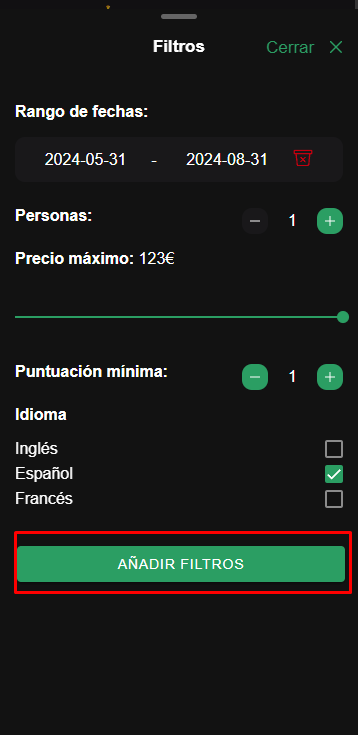
\includegraphics[width=0.3\textwidth]{7-Construccion/Manuales/mobile/aplicar filtro.png}
	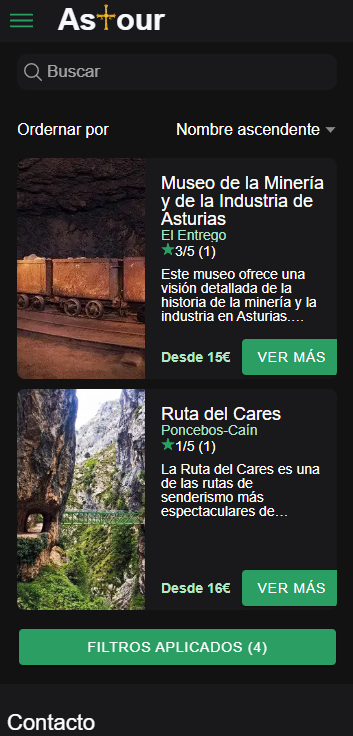
\includegraphics[width=0.3\textwidth]{7-Construccion/Manuales/mobile/lista filtrada de actividades.png}
	\caption{Explorar actividades - Filtros aplicados.}
\end{figure}

Una vez aplicados los filtros deseados, se mostrarán las actividades que coincidan con los filtros aplicados.
Y en caso de que desees hacer modificaciones o borrar los filtros, deberás pulsar el botón “Filtros aplicados (*)” que se encuentra en la parte inferior de la pantalla.
\begin{figure}[H]
	\centering
	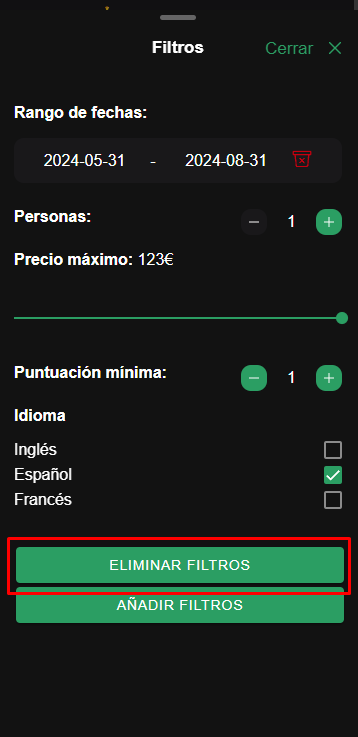
\includegraphics[width=0.3\textwidth]{7-Construccion/Manuales/mobile/eliminar filtros.png}
	\caption{Explorar actividades - Eliminar filtros.}
\end{figure}

\subsubsection{Ver Información Detallada de una Actividad}
Para ver la información detallada de una actividad, toca el botón “Ver más” de la actividad deseada.
Se abrirá una nueva ventana con la información detallada de la actividad, incluyendo el nombre, la descripción, la duración, la puntuación y la ubicación.
\begin{figure}[H]
	\centering
	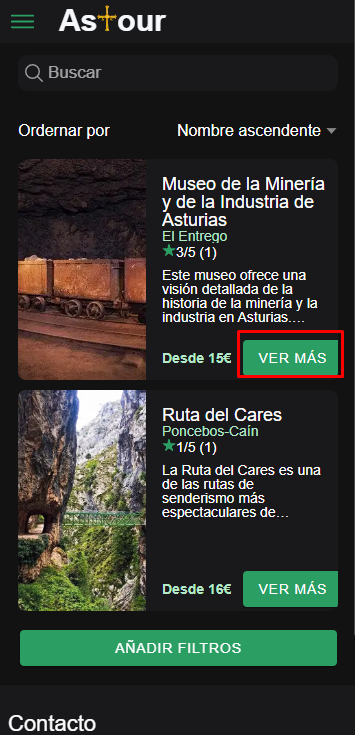
\includegraphics[width=0.3\textwidth]{7-Construccion/Manuales/mobile/ver mas.png}
	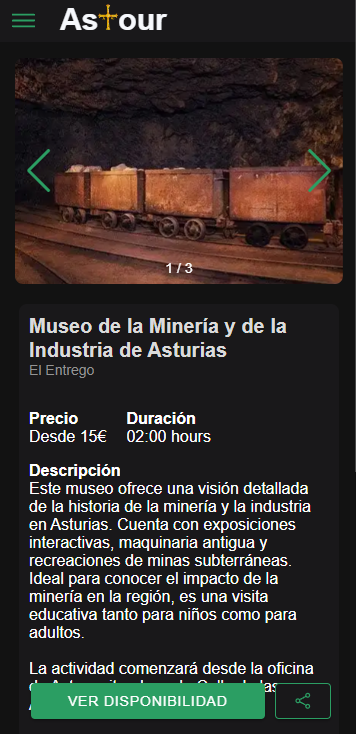
\includegraphics[width=0.3\textwidth]{7-Construccion/Manuales/mobile/detalles.png}
	\caption{Detalles de la actividad - Redirección a la información }
\end{figure}

Para ver los precios, idiomas y horarios de la actividad, toca el botón “Ver disponibilidad” que se encuentra bajo la descripción de la actividad.
Podrás seleccionar la fecha en el calendario y el número de personas usando los botones de incremento y decremento.
Una vez seleccionada la fecha y el número de personas, podrás ver los precios, idiomas y horarios disponibles para la actividad.
\begin{figure}[H]
	\centering
	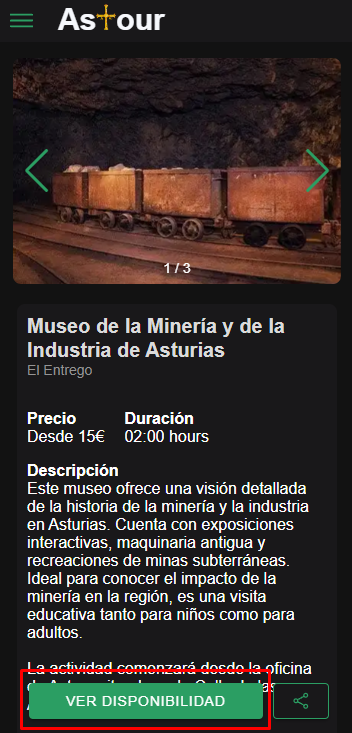
\includegraphics[width=0.3\textwidth]{7-Construccion/Manuales/mobile/ver disponibilidad.png}
	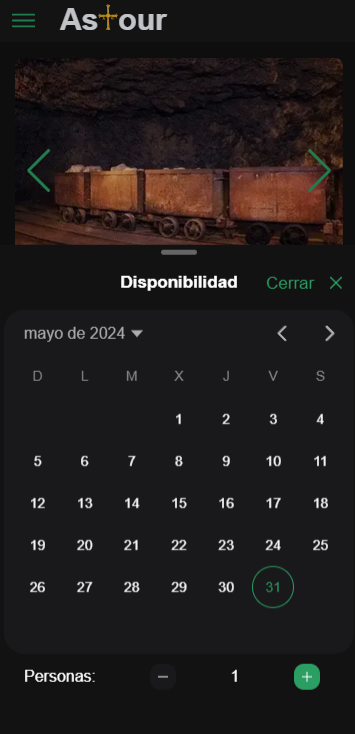
\includegraphics[width=0.3\textwidth]{7-Construccion/Manuales/mobile/disponibilidad.png}
	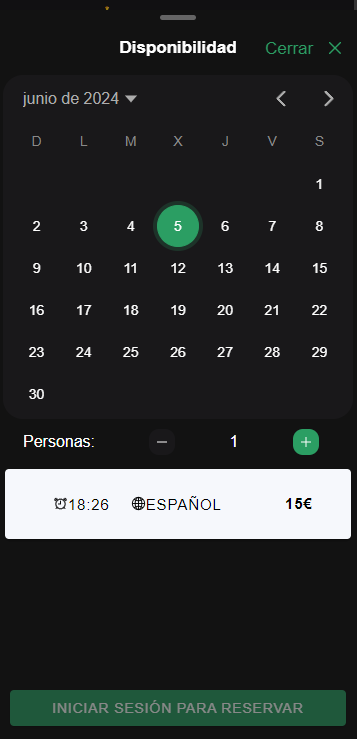
\includegraphics[width=0.3\textwidth]{7-Construccion/Manuales/mobile/fecha seleccionada.png}
	\caption{Detalles de la actividad - Ver precios, idiomas y horarios.}
\end{figure}

\subsubsection{Ver eventos proximos}
Para ver los eventos que tendrás próximamente, deberás pulsa el icono de menú en la parte superior izquierda de la página de inicio y seleccionar la opción “Eventos próximos” .
\begin{figure}[H]
	\centering
	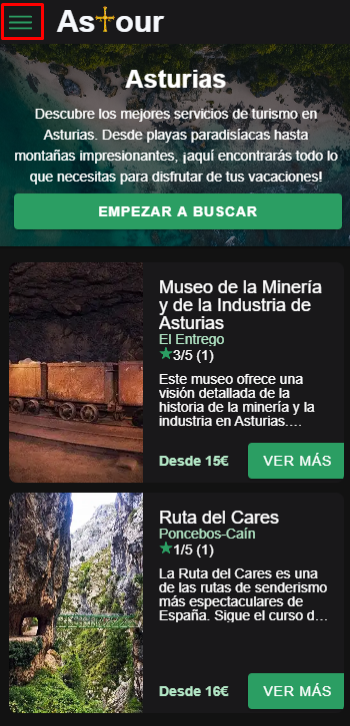
\includegraphics[width=0.3\textwidth]{7-Construccion/Manuales/mobile/menu marcado.png}
	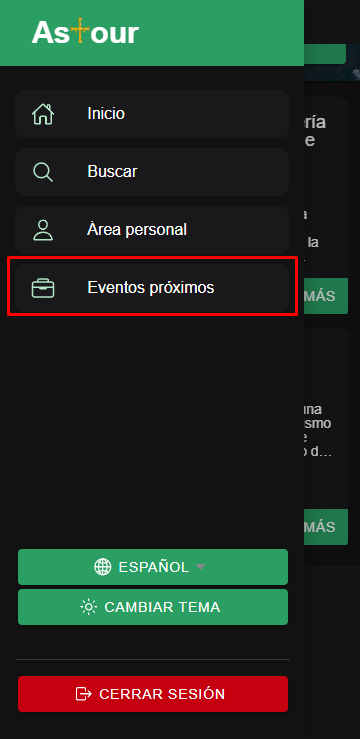
\includegraphics[width=0.3\textwidth]{7-Construccion/Manuales/mobile/eventos proximos marcado.png}
	\caption{Eventos próximos - Despliegue del menú y selección de la opción “Eventos próximos”.}
\end{figure}
Se abrirá una página donde podrás seleccionar la fecha deseada para ver los eventos programados para ese día.
Después de seleccionar el día, se mostrará lista con los eventos programados para la fecha seleccionada, incluyendo el nombre, la descripción, la duración, la ubicación y el horario.
\begin{figure}[H]
	\centering
	\includegraphics[width=0.24\textwidth]{7-Construccion/Manuales/mobile/botón calendario eventos.png}
	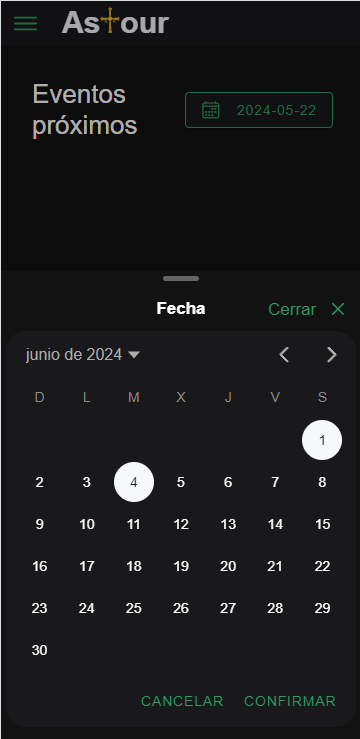
\includegraphics[width=0.24\textwidth]{7-Construccion/Manuales/mobile/calendario eventos.png}
	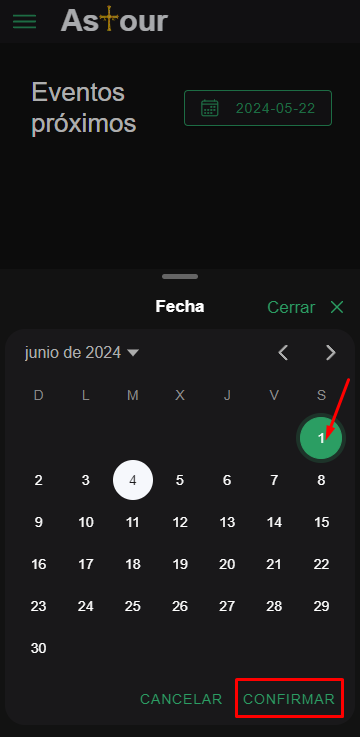
\includegraphics[width=0.24\textwidth]{7-Construccion/Manuales/mobile/seleccion dia eventos.png}
	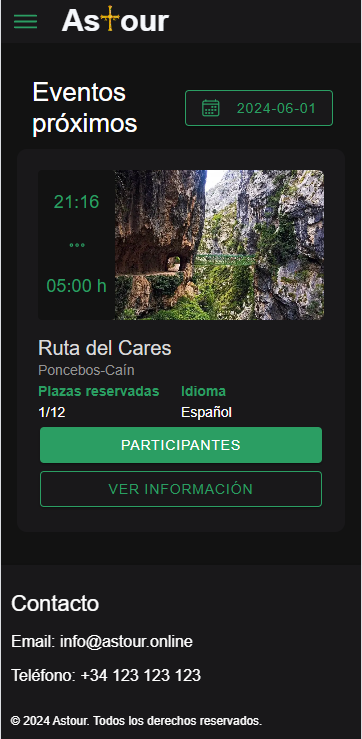
\includegraphics[width=0.24\textwidth]{7-Construccion/Manuales/mobile/eventos.png}
	\caption{Eventos próximos - Selección de la fecha y visualización de los eventos programados.}
\end{figure}
Para ver la lista de los participantes de un evento, toca el botón “Ver participantes” del evento deseado.
Se abrirá una nueva ventana con la lista de los participantes del evento, incluyendo el nombre y el número de reservas a su nombre.
\begin{figure}[H]
	\centering
	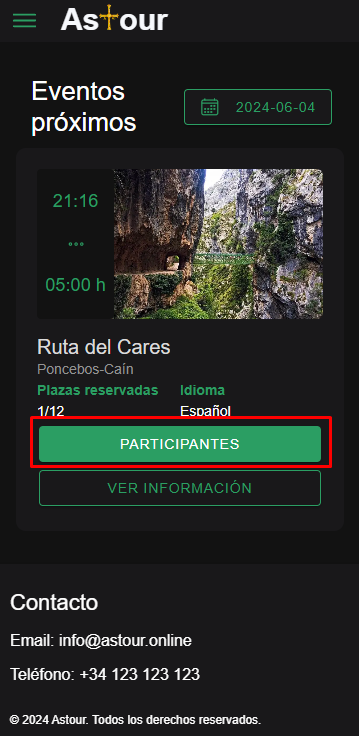
\includegraphics[width=0.3\textwidth]{7-Construccion/Manuales/mobile/participantes.png}
	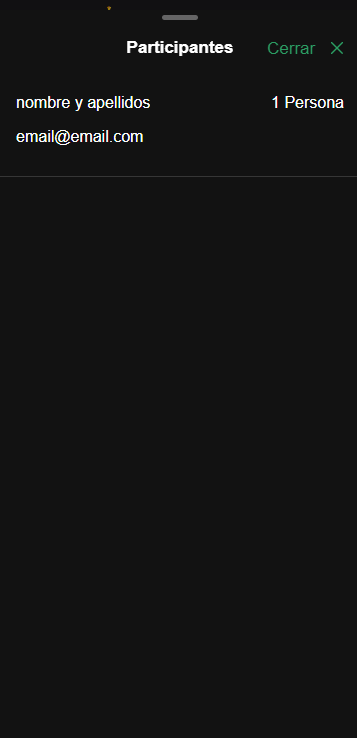
\includegraphics[width=0.3\textwidth]{7-Construccion/Manuales/mobile/lista participantes.png}
	\caption{Eventos próximos - Ver participantes de un evento.}
\end{figure}

\subsubsection{Cambiar Datos Personales}
Para cambiar tus datos personales desde tu dispositivo móvil, una vez hayas iniciado sesión, sigue estos pasos:
\begin{enumerate}
	\item Toca el ícono de menú en la parte superior izquierda de la página de inicio y selecciona la opción “Área personal” .
	      \begin{figure}[H]
		      \centering
		      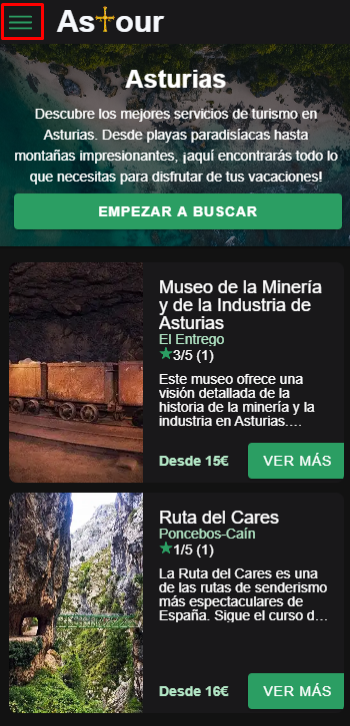
\includegraphics[width=0.3\textwidth]{7-Construccion/Manuales/mobile/menu marcado.png}
		      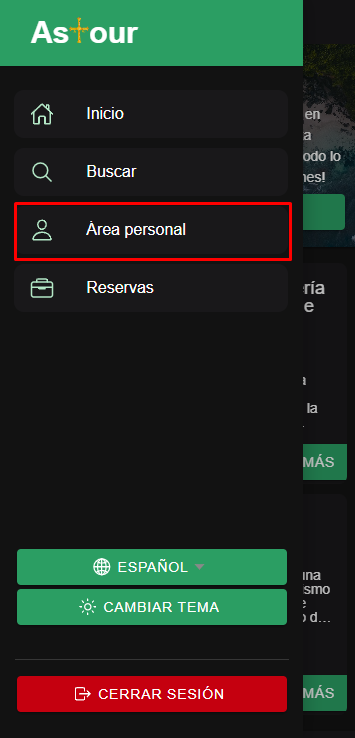
\includegraphics[width=0.3\textwidth]{7-Construccion/Manuales/mobile/area personal marcado.png}
		      \caption{Perfil - Despliegue del menú y selección de la opción “Área personal”.}
	      \end{figure}
	\item Se abrirá una página con tus datos personales y varios botones de acción. Toca el botón “Editar perfil” para acceder al formulario de edición de datos personales.
	      \begin{figure}[H]
		      \centering
		      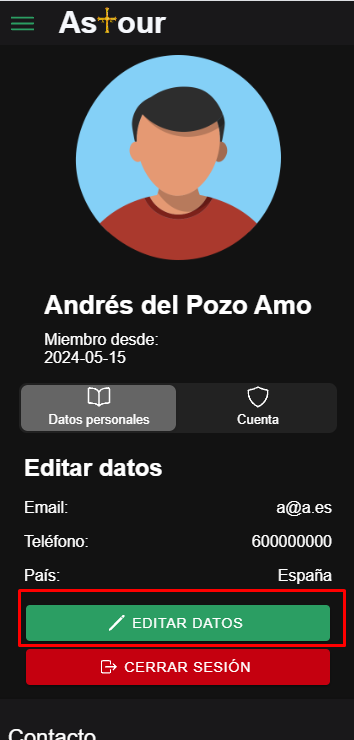
\includegraphics[width=0.3\textwidth]{7-Construccion/Manuales/mobile/editar datos.png}
		      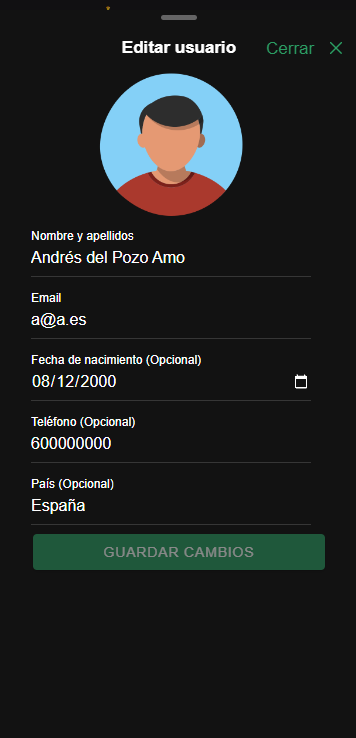
\includegraphics[width=0.3\textwidth]{7-Construccion/Manuales/mobile/formulario perfil.png}
		      \caption{Perfil - Edición de datos personales.}
	      \end{figure}
	\item Completa el formulario con los nuevos datos y toca el botón “Guardar cambios” para enviar el formulario.
	\item En el caso de querer modificar la contraseña o eliminar la cuenta habrá que hacer click en la pestaña “Cuenta”.
	      \begin{figure}[H]
		      \centering
		      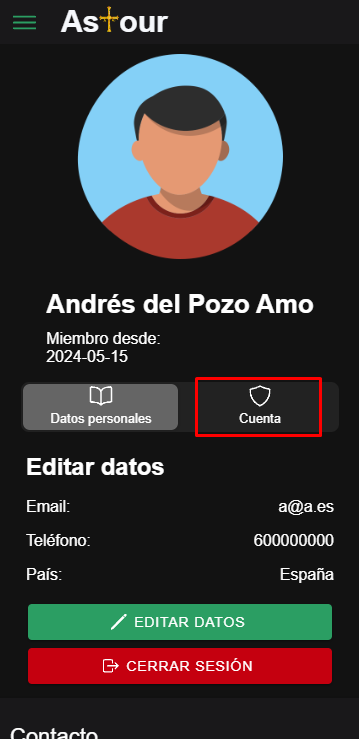
\includegraphics[width=0.3\textwidth]{7-Construccion/Manuales/mobile/apartado cuenta seleccionado.png}
		      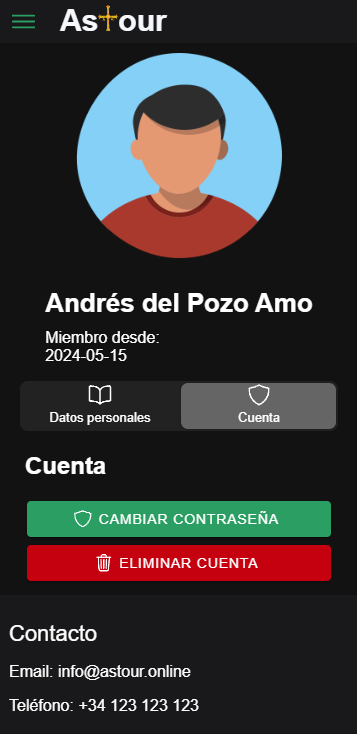
\includegraphics[width=0.3\textwidth]{7-Construccion/Manuales/mobile/editar cuenta.png}
		      \caption{Perfil - Apartado cuenta}
	      \end{figure}
	\item Toca el botón “Cambiar contraseña” para acceder al formulario de cambio de contraseña, completa el formulario con los nuevos datos y toca el botón “Guardar cambios” para enviar el formulario.
	      \begin{figure}[H]
		      \centering
		      \includegraphics[width=0.3\textwidth]{7-Construccion/Manuales/mobile/cambiar contraseña.png}
		      \includegraphics[width=0.3\textwidth]{7-Construccion/Manuales/mobile/formulario contraseña.png}
		      \caption{Perfil - Cambio de contraseña}
	      \end{figure}
	\item Toca el botón “Eliminar cuenta” para eliminar tu cuenta de la aplicación. Se abrirá una ventana de confirmación de la eliminación de la cuenta. Toca el botón “Confirmar” para eliminar tu cuenta.
	      \begin{figure}[H]
		      \centering
		      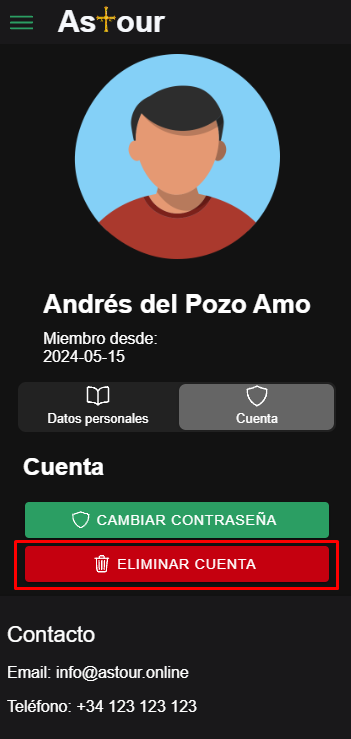
\includegraphics[width=0.3\textwidth]{7-Construccion/Manuales/mobile/eliminar cuenta.png}
		      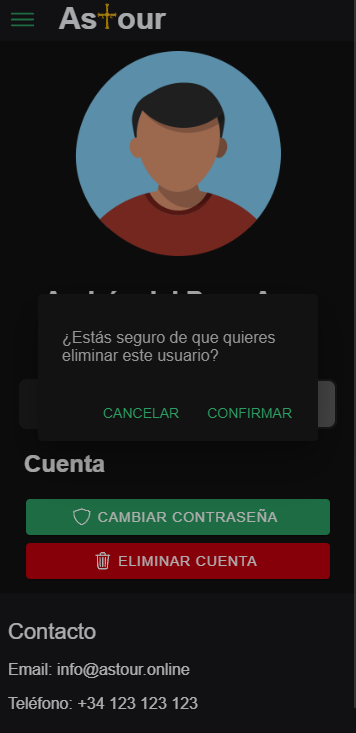
\includegraphics[width=0.3\textwidth]{7-Construccion/Manuales/mobile/confirmar eliminacion cuenta.png}
		      \caption{Perfil - Eliminar cuenta}
	      \end{figure}
\end{enumerate}

\subsubsection{Cerrar Sesión}
Para poder cerrar sesión debes estar previamente logueado en la aplicación. Si no lo estás deberás hacerlo siguiendo los pasos descritos en la sección “Inicio de Sesión” .
\\ \\[1ex]
Para cerrar sesión desde tu dispositivo móvil, toca el ícono de menú en la parte superior izquierda de la página de inicio y selecciona la opción “Cerrar sesión” .
\begin{figure}[H]
	\centering
	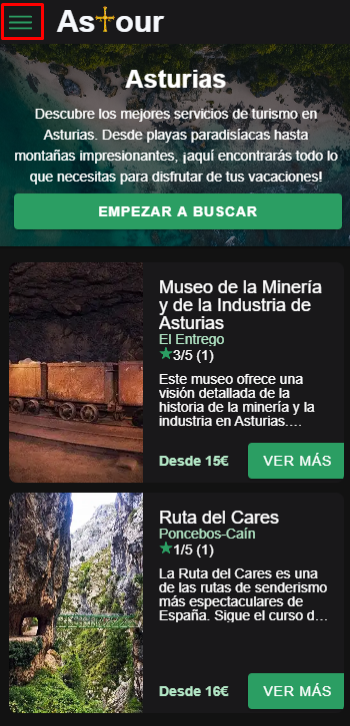
\includegraphics[width=0.3\textwidth]{7-Construccion/Manuales/mobile/menu marcado.png}
	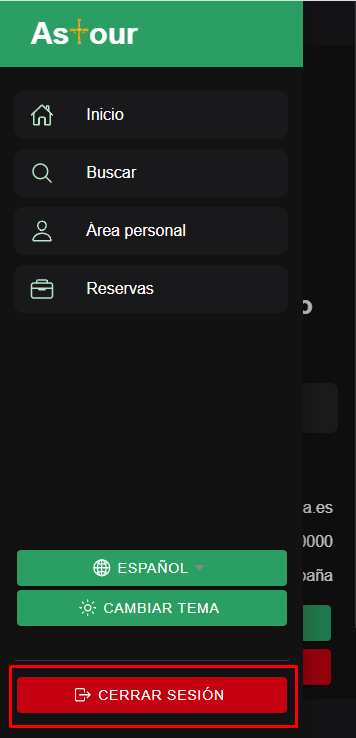
\includegraphics[width=0.3\textwidth]{7-Construccion/Manuales/mobile/cerrar sesion marcado.png}
	\caption{Cerrar sesión - Despliegue del menú y selección de la opción “Cerrar sesión”.}
\end{figure}
Se te redirigirá a la página de inicio y habrás cerrado sesión con éxito. Si deseas volver a iniciar sesión, sigue los pasos descritos en la sección “Inicio de Sesión” .

\subsubsection{Cambiar Idioma}
Para cambiar el idioma de la página web desde tu dispositivo móvil, sigue estos pasos:
\begin{enumerate}
	\item Toca el ícono de menú en la parte superior izquierda de la página de inicio y selecciona la opción, en este caso, “Español” . El contenido del botón puede variar dependiendo del idioma actual.
	      \begin{figure}[H]
		      \centering
		      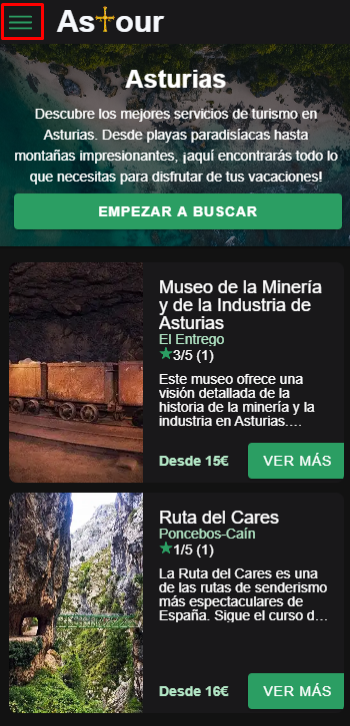
\includegraphics[width=0.3\textwidth]{7-Construccion/Manuales/mobile/menu marcado.png}
		      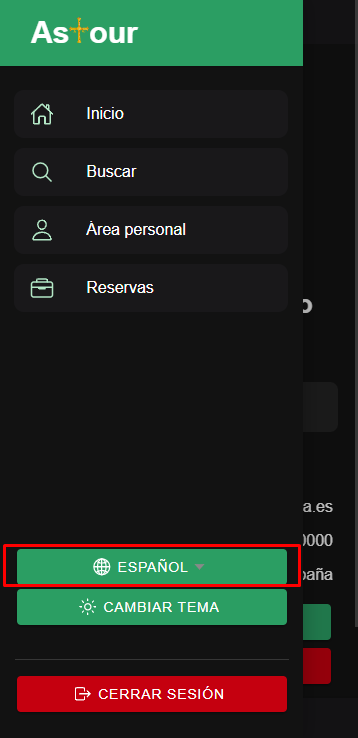
\includegraphics[width=0.3\textwidth]{7-Construccion/Manuales/mobile/idioma marcado.png}
		      \caption{Cambiar idioma - Despliegue del menú y selección de la opción “Español”.}
	      \end{figure}
	\item Se abrirá un menú desplegable con una lista de idiomas disponibles. Toca el idioma deseado para cambiar el idioma de la página web.
	      La página web se actualizará automáticamente con el idioma seleccionado.
	      \begin{figure}[H]
		      \centering
		      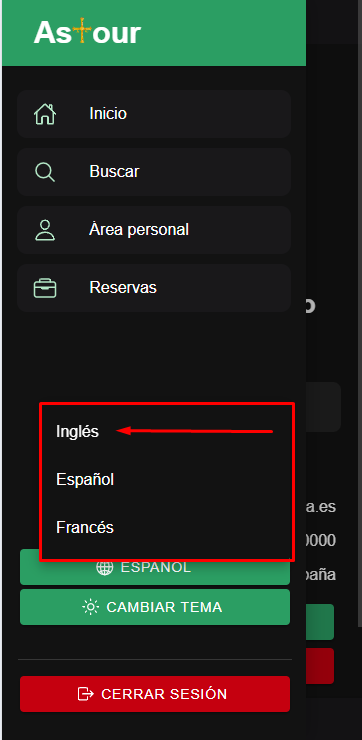
\includegraphics[width=0.3\textwidth]{7-Construccion/Manuales/mobile/opciones idioma.png}
		      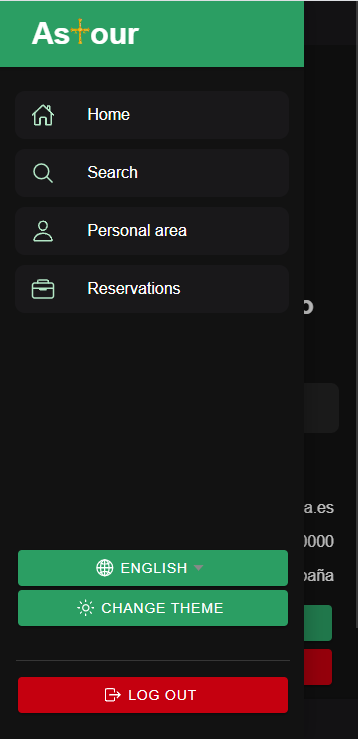
\includegraphics[width=0.3\textwidth]{7-Construccion/Manuales/mobile/ingles.png}
		      \caption{Cambiar idioma - Cambio de idioma.}
	      \end{figure}
\end{enumerate}

\subsubsection{Cambiar Tema}
\begin{enumerate}
	\item Toca el ícono de menú en la parte superior izquierda de la página de inicio y selecciona la opción “Cambiar tema” .
	      \begin{figure}[H]
		      \centering
		      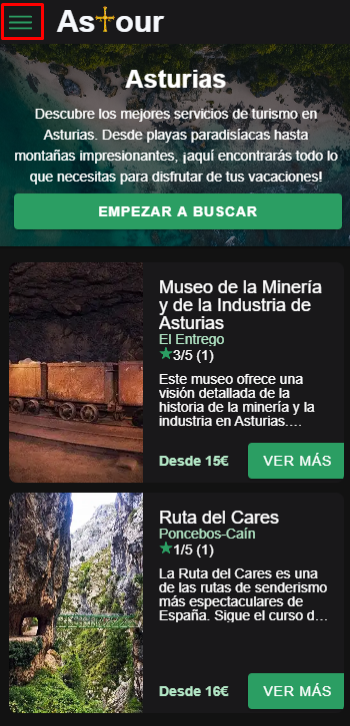
\includegraphics[width=0.3\textwidth]{7-Construccion/Manuales/mobile/menu marcado.png}
		      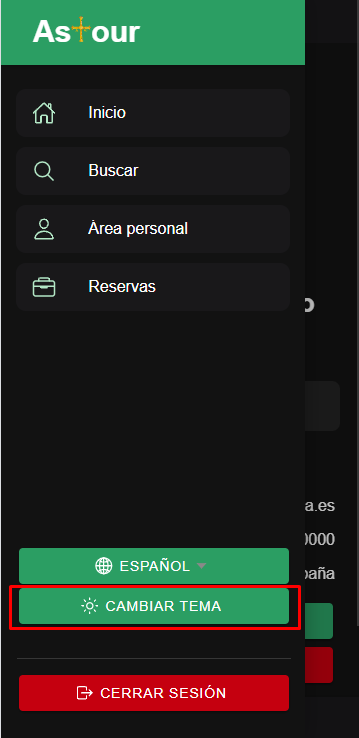
\includegraphics[width=0.3\textwidth]{7-Construccion/Manuales/mobile/tema marcado.png}
		      \caption{Cambiar tema - Despliegue del menú y selección de la opción “Cambiar tema”.}
	      \end{figure}
	\item La página web se actualizará automáticamente con el tema contrario. Si el tema actual es claro, se cambiará a oscuro y viceversa.
	      El icono de la opción de tema, del menú superior, cambiará al tema contrario. Si el tema actual es claro, se cambiará a una luna y si el tema actual es oscuro, se cambiará a un sol.
	      \begin{figure}[H]
		      \centering
		      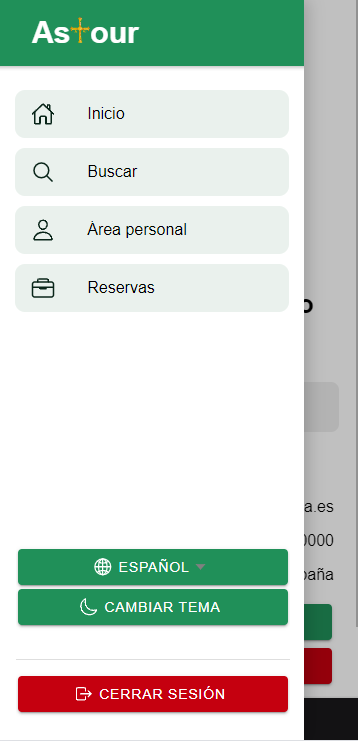
\includegraphics[width=0.3\textwidth]{7-Construccion/Manuales/mobile/tema claro.png}
		      \caption{Cambiar tema - Cambio de tema.}
	      \end{figure}
\end{enumerate}

\subsubsection{Soporte Técnico}
Si encuentras algún problema o tienes alguna pregunta relacionada con el uso de nuestra página web, no dudes en contactar a nuestro equipo de soporte técnico.
Puedes encontrar la información de contacto en el apartado “Contacto” de la parte inferior de la página.
\begin{figure}[H]
	\centering
	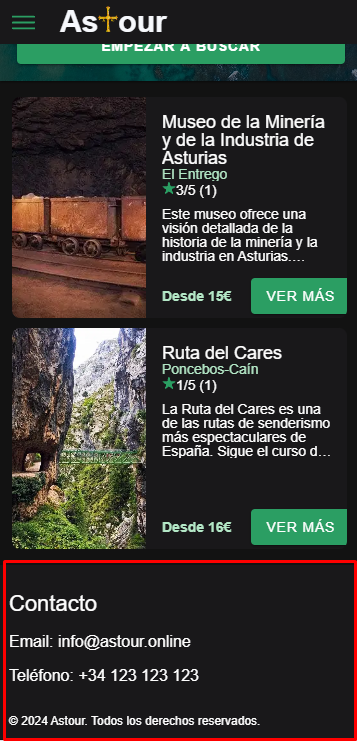
\includegraphics[width=0.3\textwidth]{7-Construccion/Manuales/mobile/contacto.png}
	\caption{Contacto - Información de contacto.}
\end{figure}